\section{About the EROS training set}

We use a training data set provided by \citet{kim2014} which contains labels (main and sub--classes) and lightcurves for $32655$ sources in the Large Magellanic Cloud (LMC). The lightcurves were recorded by the Expérience pour la Recherche d’Objets Sombres (EROS) project, a wide--field survey. A thorough description of the compilation process is available in \citet{kim2014}, however, here is a list of the main steps:

\begin{enumerate}
\item Compile known periodoic variables in the LMC from the OGLE and MACHO surveys
\item Add $982$ blue variables (BVs) from the MACHO database
\item Add 565 quasi--stellar objects (QSOs)
\item 
\end{enumerate}

% Number of sources in the data set
% Not a standard astronomical B and R bands

\section{Feature Extraction \& Feature Selection}

We extract a variety of features characterizing the variability of the source. A lot of them are standard statistical features, but some are more sophisticated, trying to incorporate a model of the underlying physics. In the following, $N$ will be the number of data points in the light curve, $(t_i, m_i)$ the $i^{\text{th}}$ data point in the light curve.

\begin{enumerate}
%\setlength{\itemsep}{5pt}
%\setlength{\parskip}{0pt}
%\setlength{\parsep}{0pt}
%\setlength{\abovedisplayskip}{.5em}
%\setlength{\belowdisplayskip}{.5em}

\litem{$\mu$ (Mean of magnitude)} The arithmetic mean of the magnitude, given by
\begin{equation}\mu = \frac{1}{N} \sum\limits_{i=1}^{N} m_i.\end{equation}

\litem{$\sigma$ (Standard deviation of magnitude)} The standard deviation of the magnitude, given by
\begin{equation}\sigma = \sqrt{\frac{1}{N} \sum_{i=1}^N (m_i - \mu)^2}.\end{equation}

\litem{$Q_{50}$ (Median of magnitude)} The median of the magnitude, given by
\begin{equation}Q_{50} = \cdots.\end{equation}

\litem{$\bar \mu$ (Weighted mean of magnitude)} The weighted arithmetic mean of the magnitude, given by
\begin{equation}\bar \mu = \big(\sum\limits_{i=1}^{N} w_i m_i\big) \; / \; \big(\sum\limits_{i=1}^{N} w_i\big).\end{equation}
% @TODO: Specify weights

\litem{$\bar \sigma$ (Weighted standard deviation of magnitude)} The weighted standard deviation of the magnitude, given by
\begin{equation}\bar \sigma = \cdots.\end{equation}
% @TODO: Specify weights
% @TODO: Add formula for weighted standard deviation

\litem{$\gamma_1$ (Skewness)} The skewness of the magnitude, given by
\begin{equation}\gamma_1 = \cdots.\end{equation}

\litem{$\gamma_2$ (Kurtosis)} The kurtosis of the magnitude, given by
\begin{equation}\gamma_2 = \cdots.\end{equation}

\litem{$Q_{25}$ (25\% quartile)} The 25\% quartile of the magnitude, given by
\begin{equation}Q_{25} = \cdots.\end{equation}

\litem{$Q_{75}$ (75\% quartile)} The 75\% quartile of the magnitude, given by
\begin{equation}Q_{75} = \cdots.\end{equation}

\litem{$\text{IQR}$ (Interquartile range)} The interquartile range of the magnitude, given by
\begin{equation}\text{IQR} = Q_{75} -Q_{25}.\end{equation}

\litem{$P_{\text{LS}}$ (Lomb--Scargle period)} The period of the signal according to the Lomb--Scargle algorithm, given by
\begin{equation}P_{\text{LS}} = \frac{1}{2 \sigma_y^2} \Bigg\{ \frac{\big[\sum\limits_{i=1}^k (y_i - \mu_y) \cos(\omega(t_i - \tau))\big]^2}{\sum\limits_{i=1}^k \cos^2(\omega(t_i - \tau))} + \frac{\big[\sum\limits_{i=1}^k (y_i - \mu_y) \sin(\omega(t_i - \tau))\big]^2}{\sum\limits_{i=1}^k \sin^2(\omega(t_i - \tau))}\Bigg\}\end{equation}

\litem{$\text{FAP}_{\text{LS}}$ (False--Alarm probability for Lomb--Scargle)} The false--alarm probability (FAP) for the Lomb--Scargle algorithm, given by
\begin{equation}\text{FAP}_{\text{LS}}(x) = 1 - (1 - \euler^{-x})^M.\end{equation}

\litem{$\text{SNR}$ (Signal--to--noise ratio)} The signal--to--noise ratio, given by
\begin{equation}\text{SNR} = \frac{\mu}{\sigma}.\end{equation}

\litem{$S$ (Shannon entropy)} The Shannon entropy of the signal, given by
\begin{equation}S = -\sum\limits_{i=1}^N m_i \ln(m_i).\end{equation}

\litem{$\eta$ ($\cdots$)} The $\eta$ feature as proposed by \citep{}, given by
\begin{equation}\eta = \frac{1}{\sigma^2 (N-1)} \sum\limits_{i=1}^{N-1} (m_{i+1} - m_{i})^2.\end{equation}

\litem{$\cdots$ (Half--magnitude--amplitude ratio)} The ratio between higher \resp lower amplitudes than average, given by
\begin{equation}\cdots = \cdots.\end{equation}

\litem{$\text{MAD}^{(1)}$ (Mean absolute deviation)} The mean absolute deviation of the magnitude, given by
\begin{equation}\text{MAD}^{(1)} = \cdots.\end{equation}

\litem{$\text{MAD}^{(2)}$ (Median absolute deviation)} The median absolute deviation of the magnitude, given by
\begin{equation}\text{MAD}^{(2)} = \cdots.\end{equation}

\litem{$\text{SF}_A$ (Structure function $A$)} The ...
\begin{equation}\text{SF}_A = \cdots.\end{equation}

\litem{$\text{SF}_\gamma$ (Structure function $\gamma$)} The ...
\begin{equation}\text{SF}_\gamma = \cdots.\end{equation}

\litem{$\mathcal{F}$ (Fourier series)} We fit standard fourier series with five terms to the phase--folded lightcurve.
\begin{equation}\mathcal{F}(t) = \frac{A_0}{2} + \sum_{k=1}^{\infty} ( A_k \cos(2 \pi k t) + B_k \sin(2 \pi k t) ).\end{equation}

% CE – three candidate periods + scores
% sf-A-error, sf-gamma-error
% Slope percentile features
% fourier-A-i, fourier-phi-i
% fourier-residuals

% Shapiro-W und Shapiro-p
% Proper citing of all equations

\end{enumerate}

This leads to a total of $\cdots$ features in $\cdots$ bands.

% State that feature are highly correlated
% Show histogram of some features.
% Show some scatterplots
% More about period finding

\section{Performance of the Support Vector Machine}

\begin{figure}[H]
\subfigure{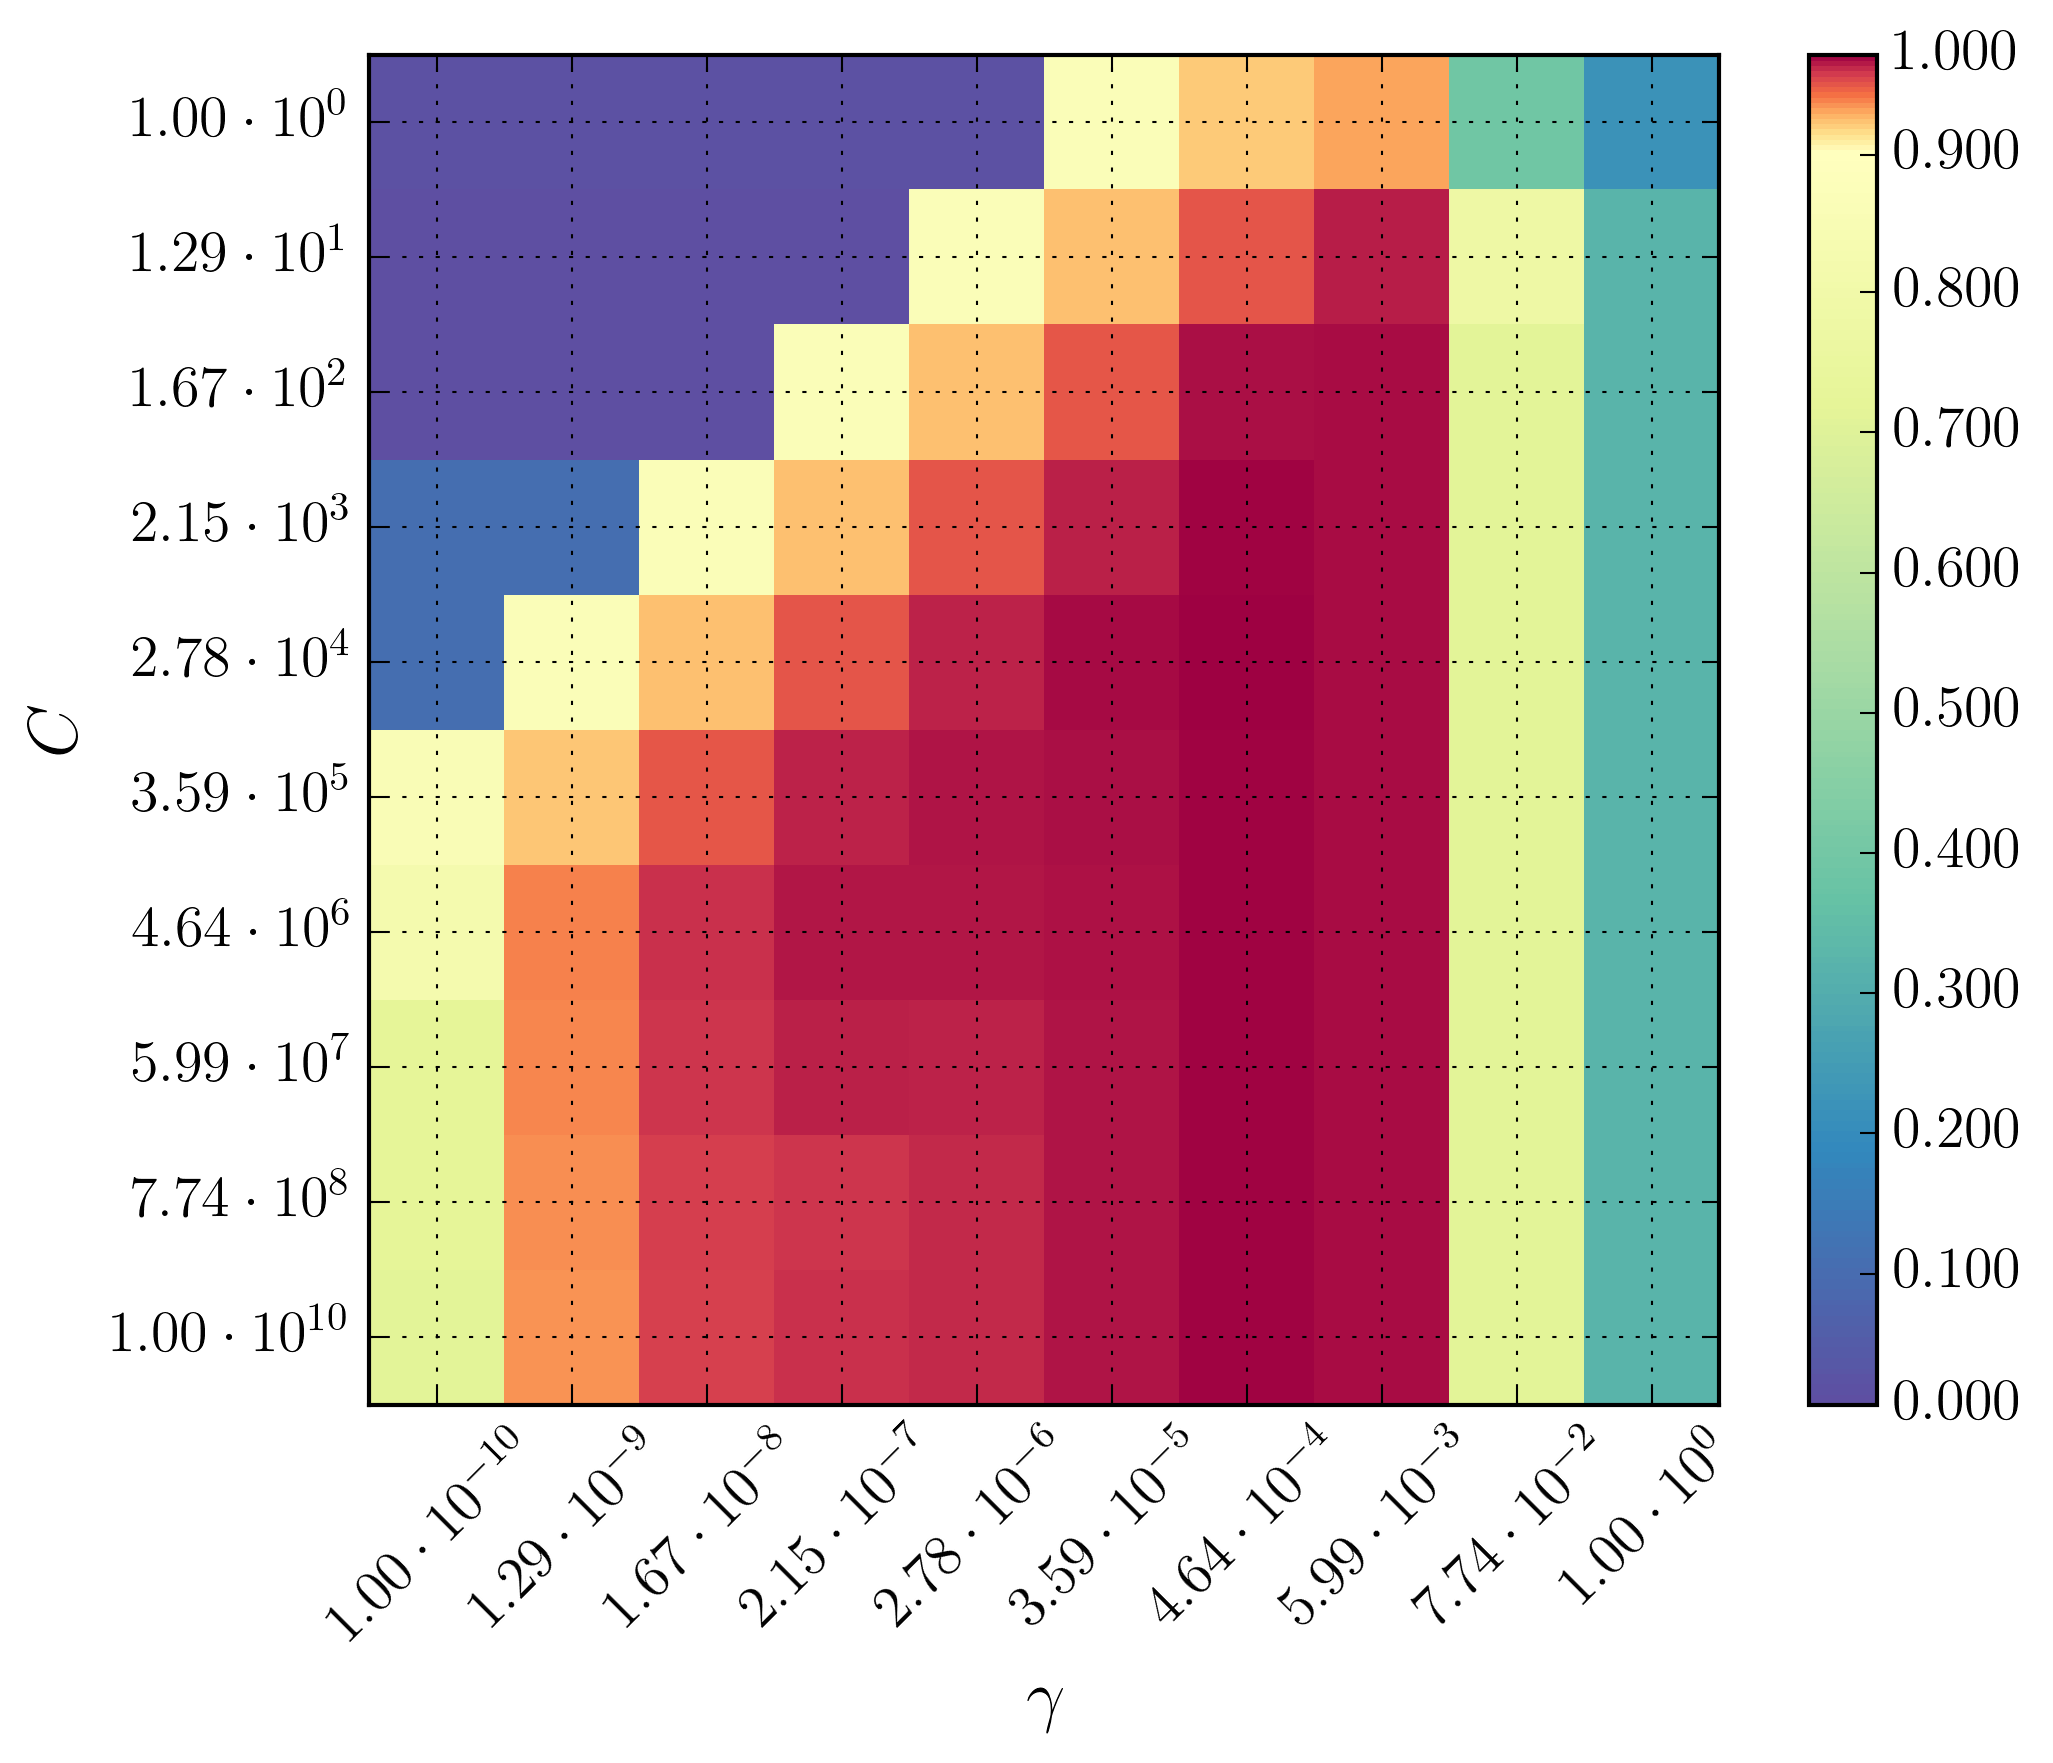
\includegraphics[width=0.49\textwidth,height=0.4\textwidth]{figures/gridsearch/svm/superclasses/svm-superclasses-01.png}}
\hfill
\subfigure{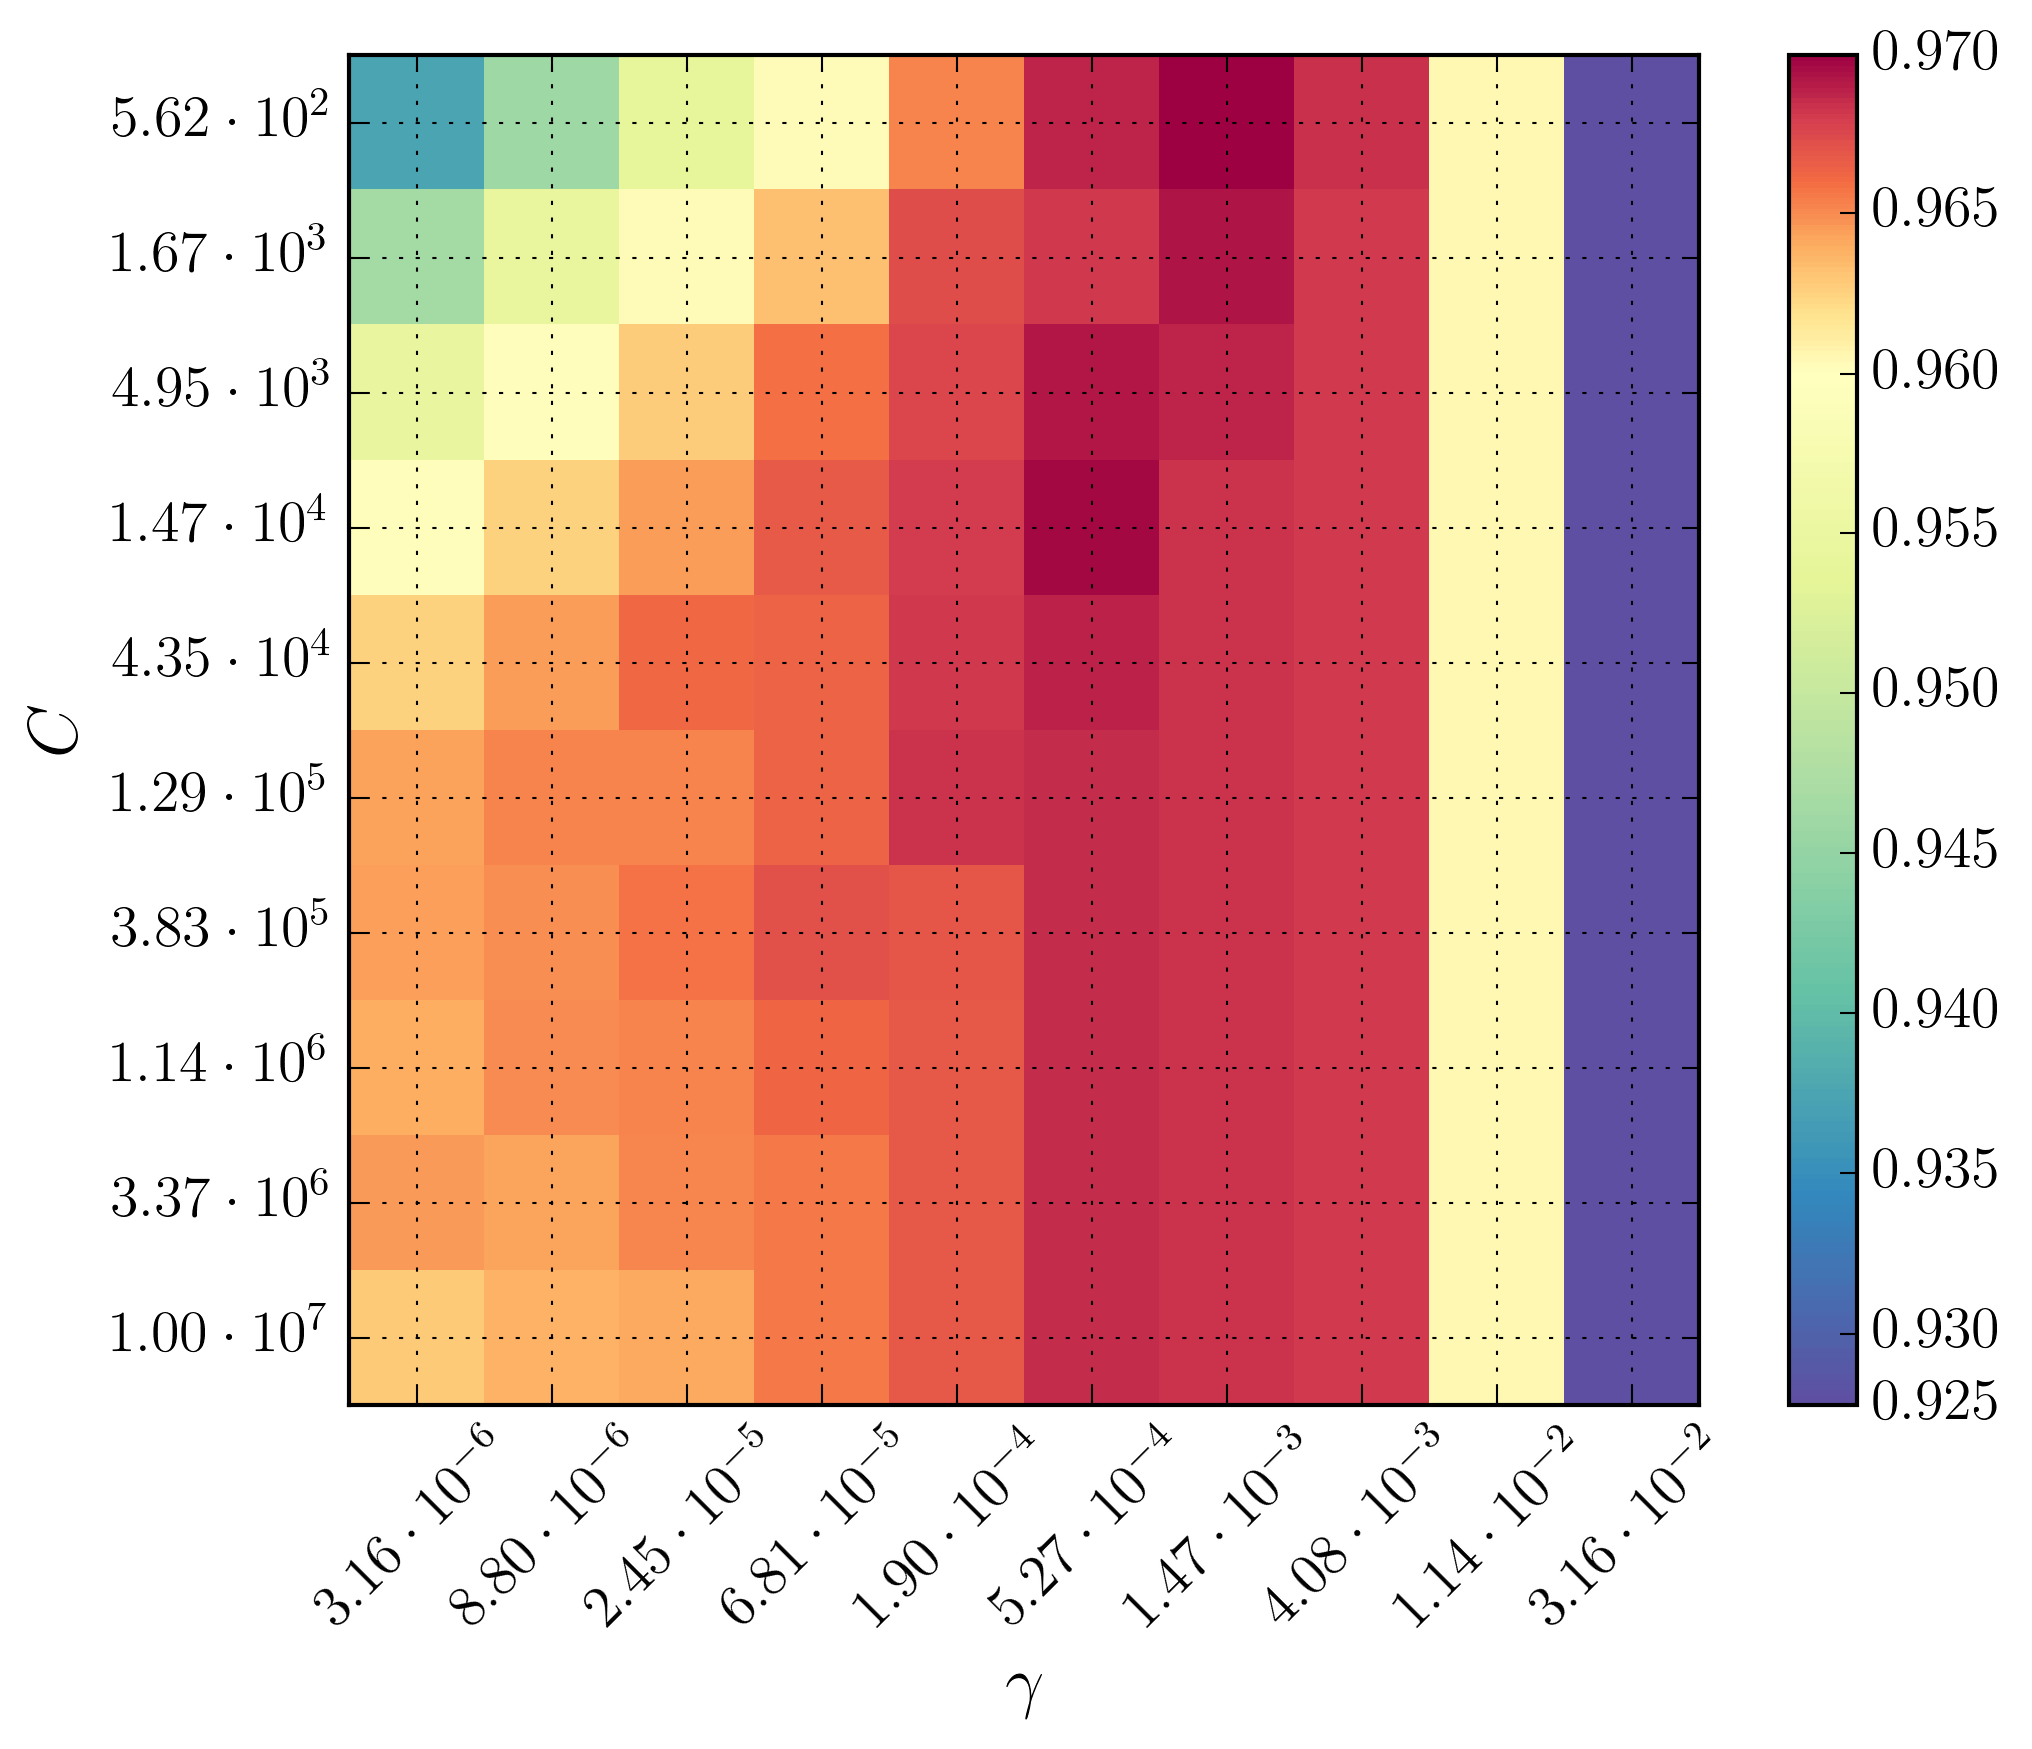
\includegraphics[width=0.51\textwidth,height=0.4\textwidth]{figures/gridsearch/svm/superclasses/svm-superclasses-02.png}}
\hfill
\subfigure{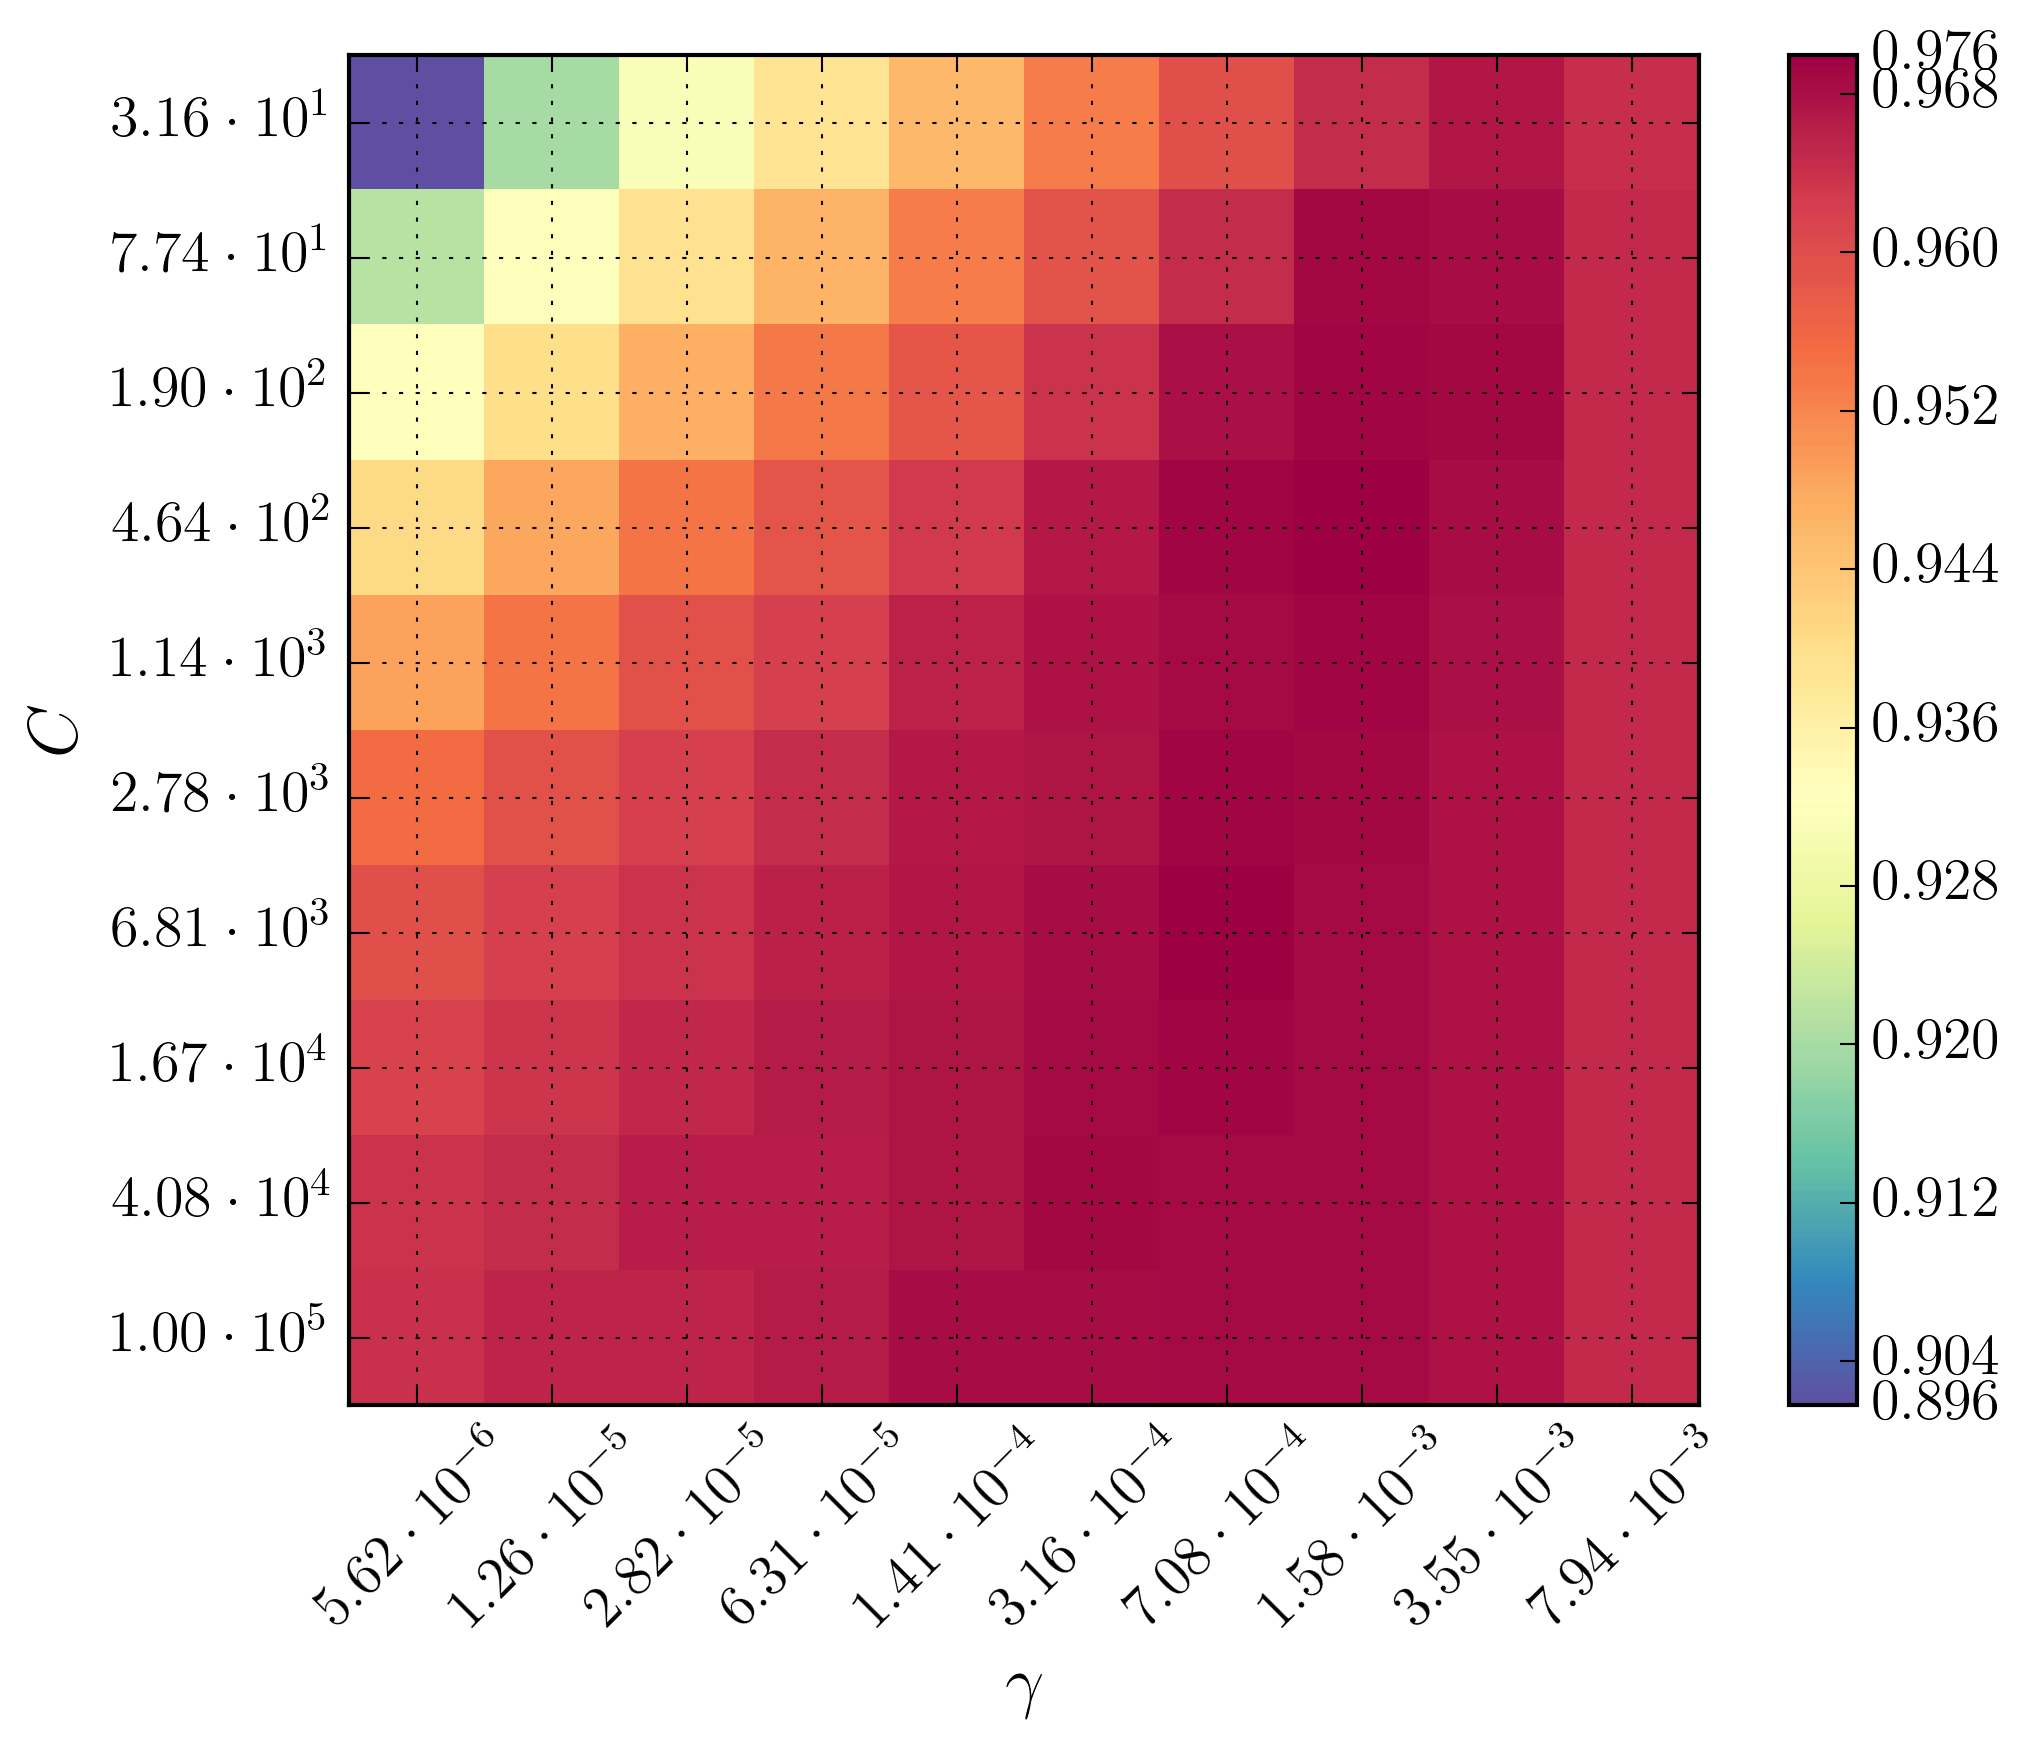
\includegraphics[width=0.49\textwidth,height=0.4\textwidth]{figures/gridsearch/svm/superclasses/svm-superclasses-03.png}}
\hfill
\subfigure{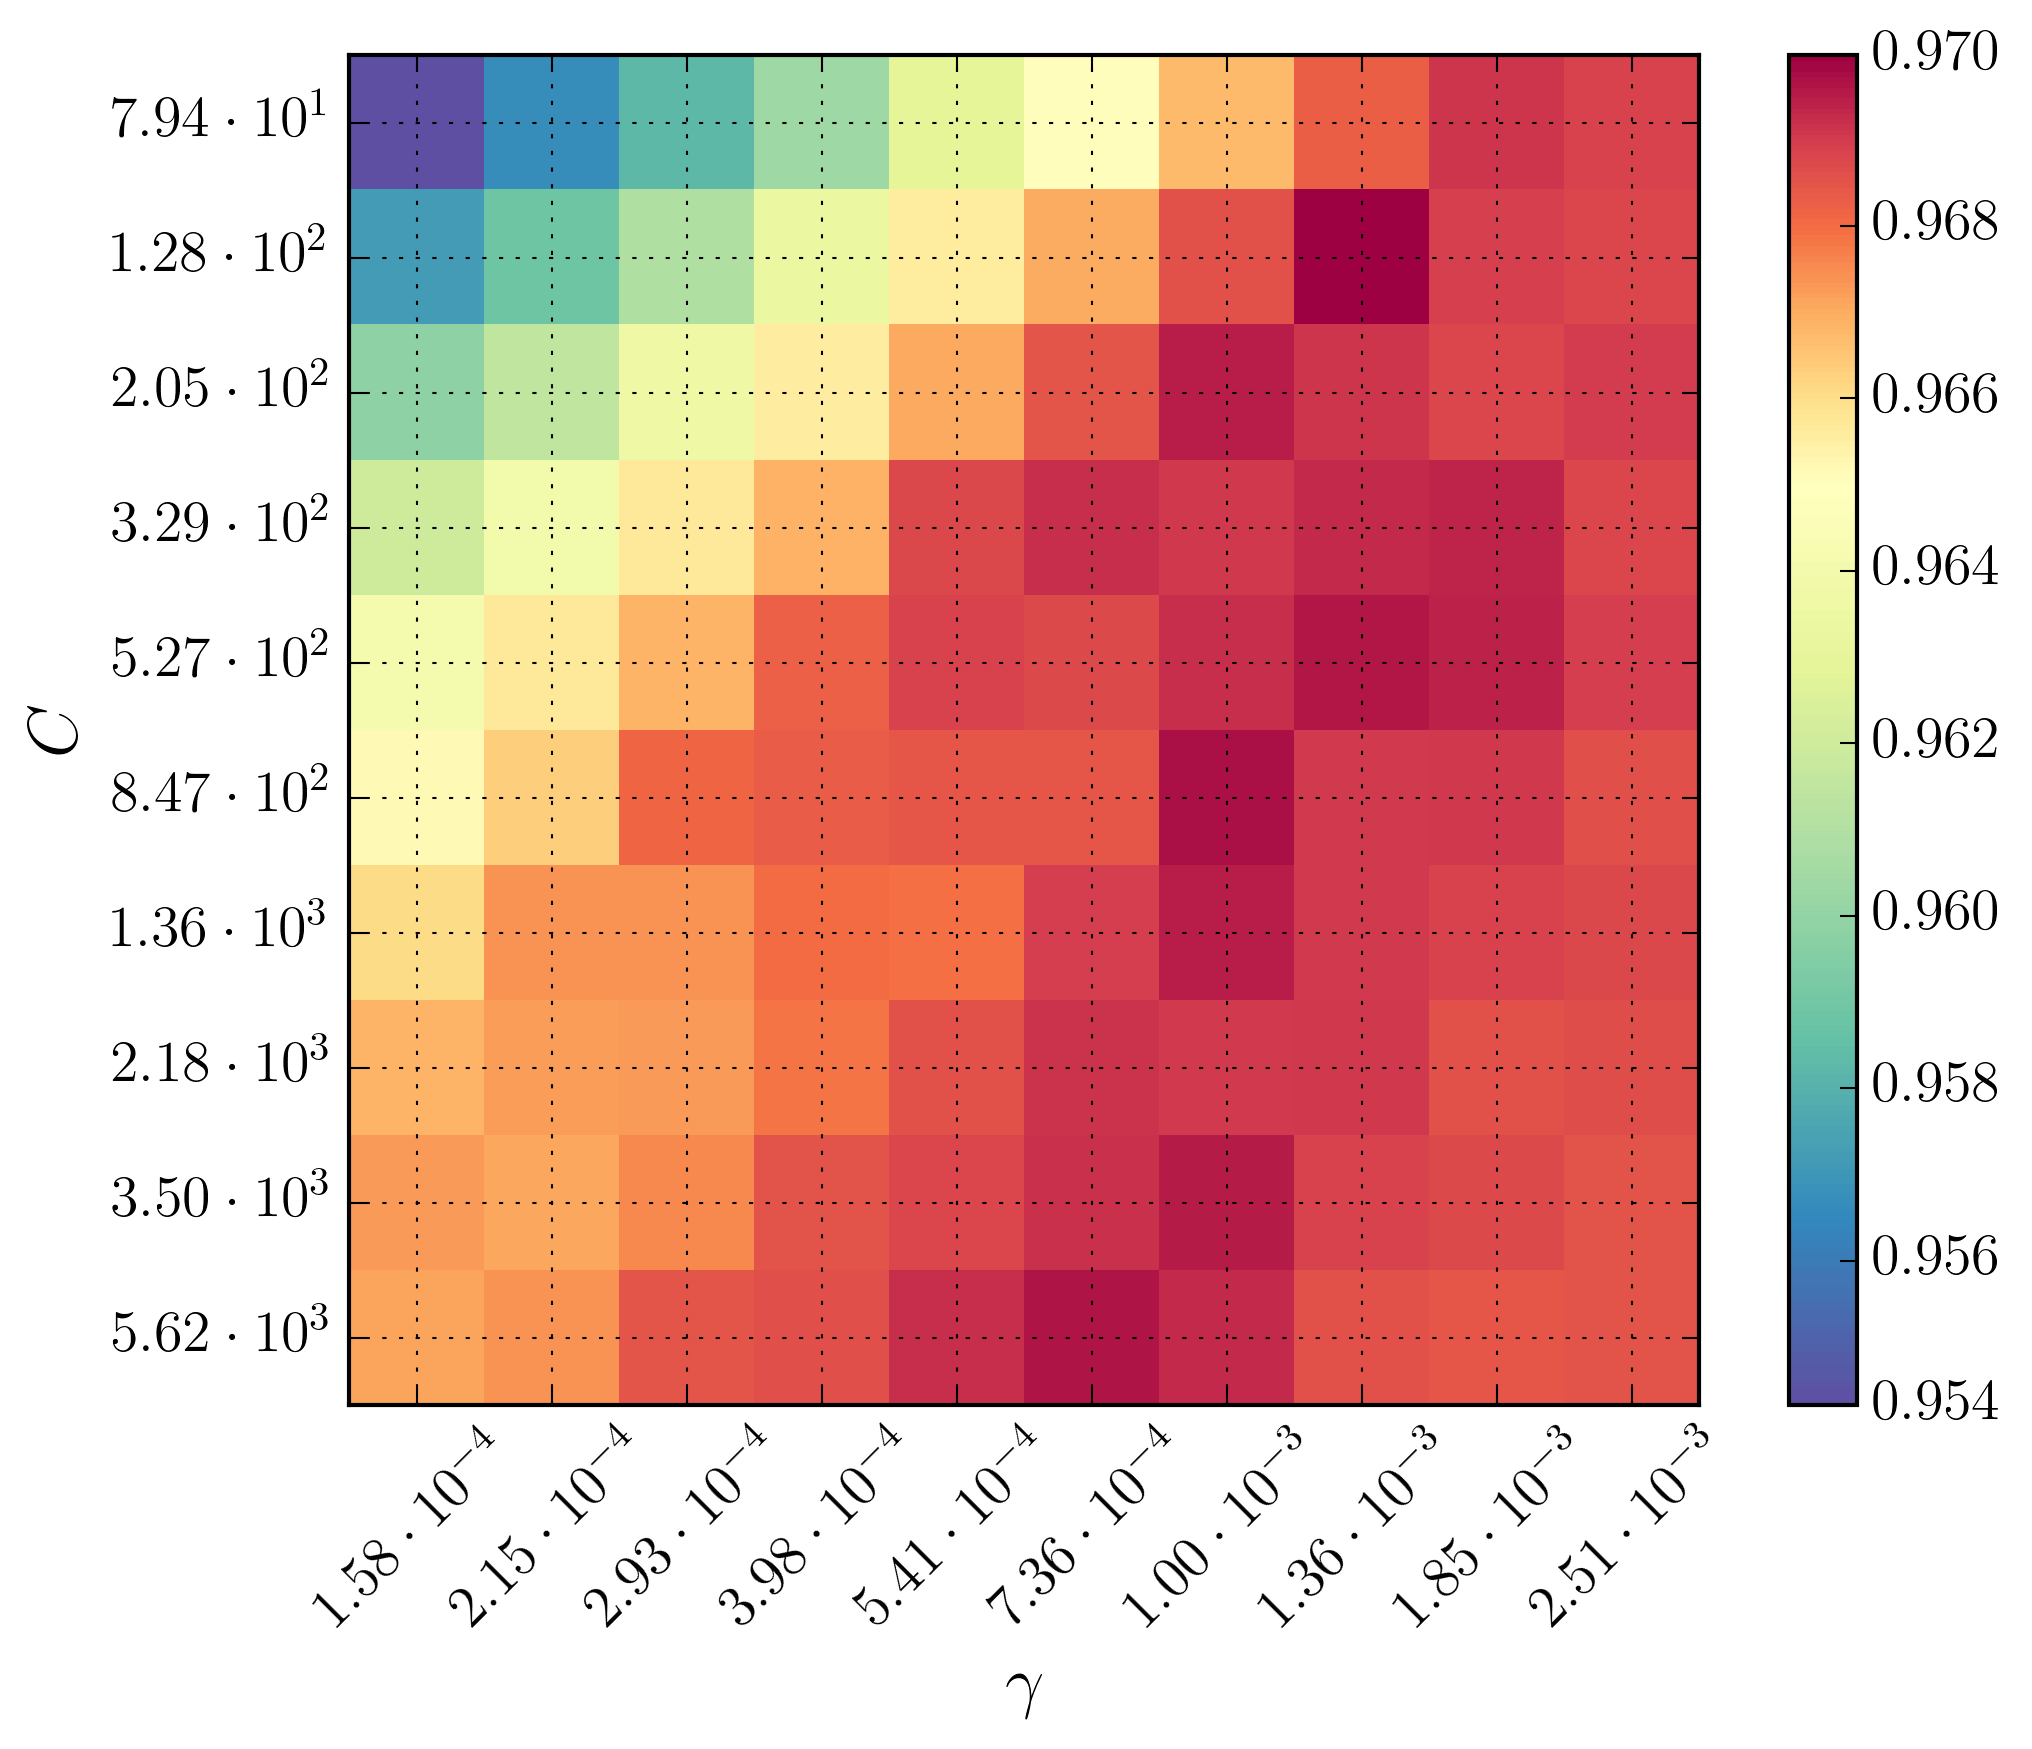
\includegraphics[width=0.51\textwidth,height=0.4\textwidth]{figures/gridsearch/svm/superclasses/svm-superclasses-04.png}}
\hfill
\subfigure{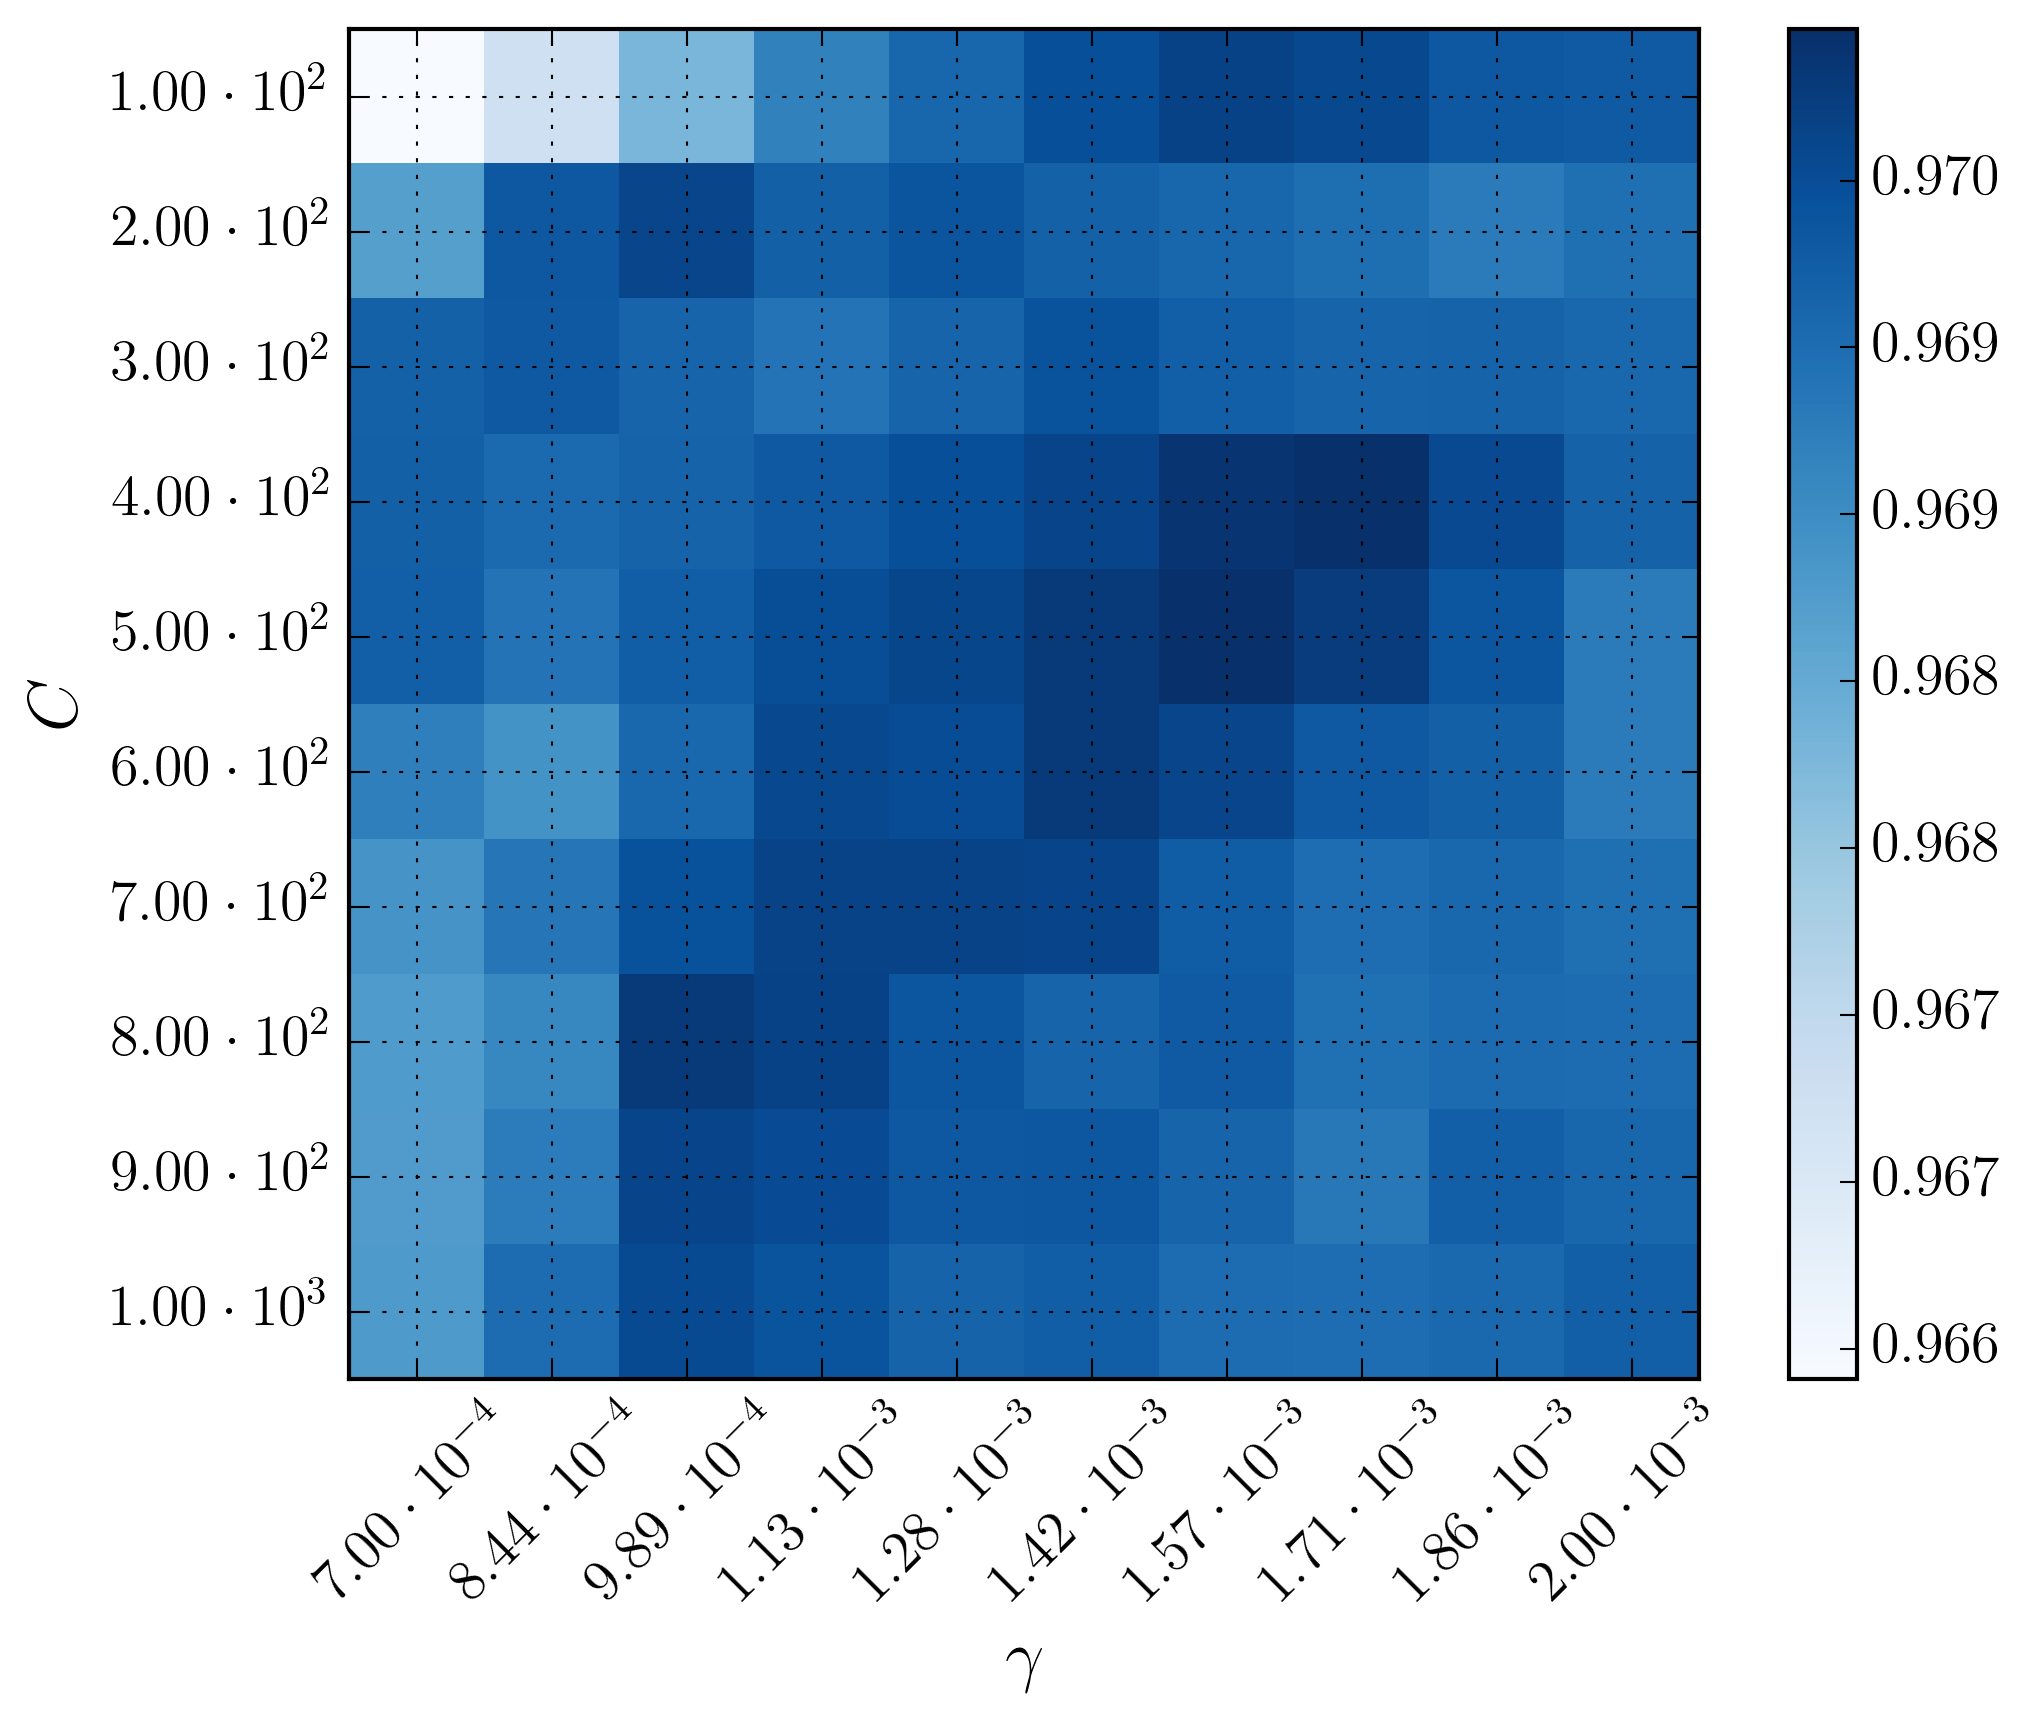
\includegraphics[width=0.49\textwidth,height=0.4\textwidth]{figures/gridsearch/svm/superclasses/svm-superclasses-05.png}}
\hfill
\subfigure{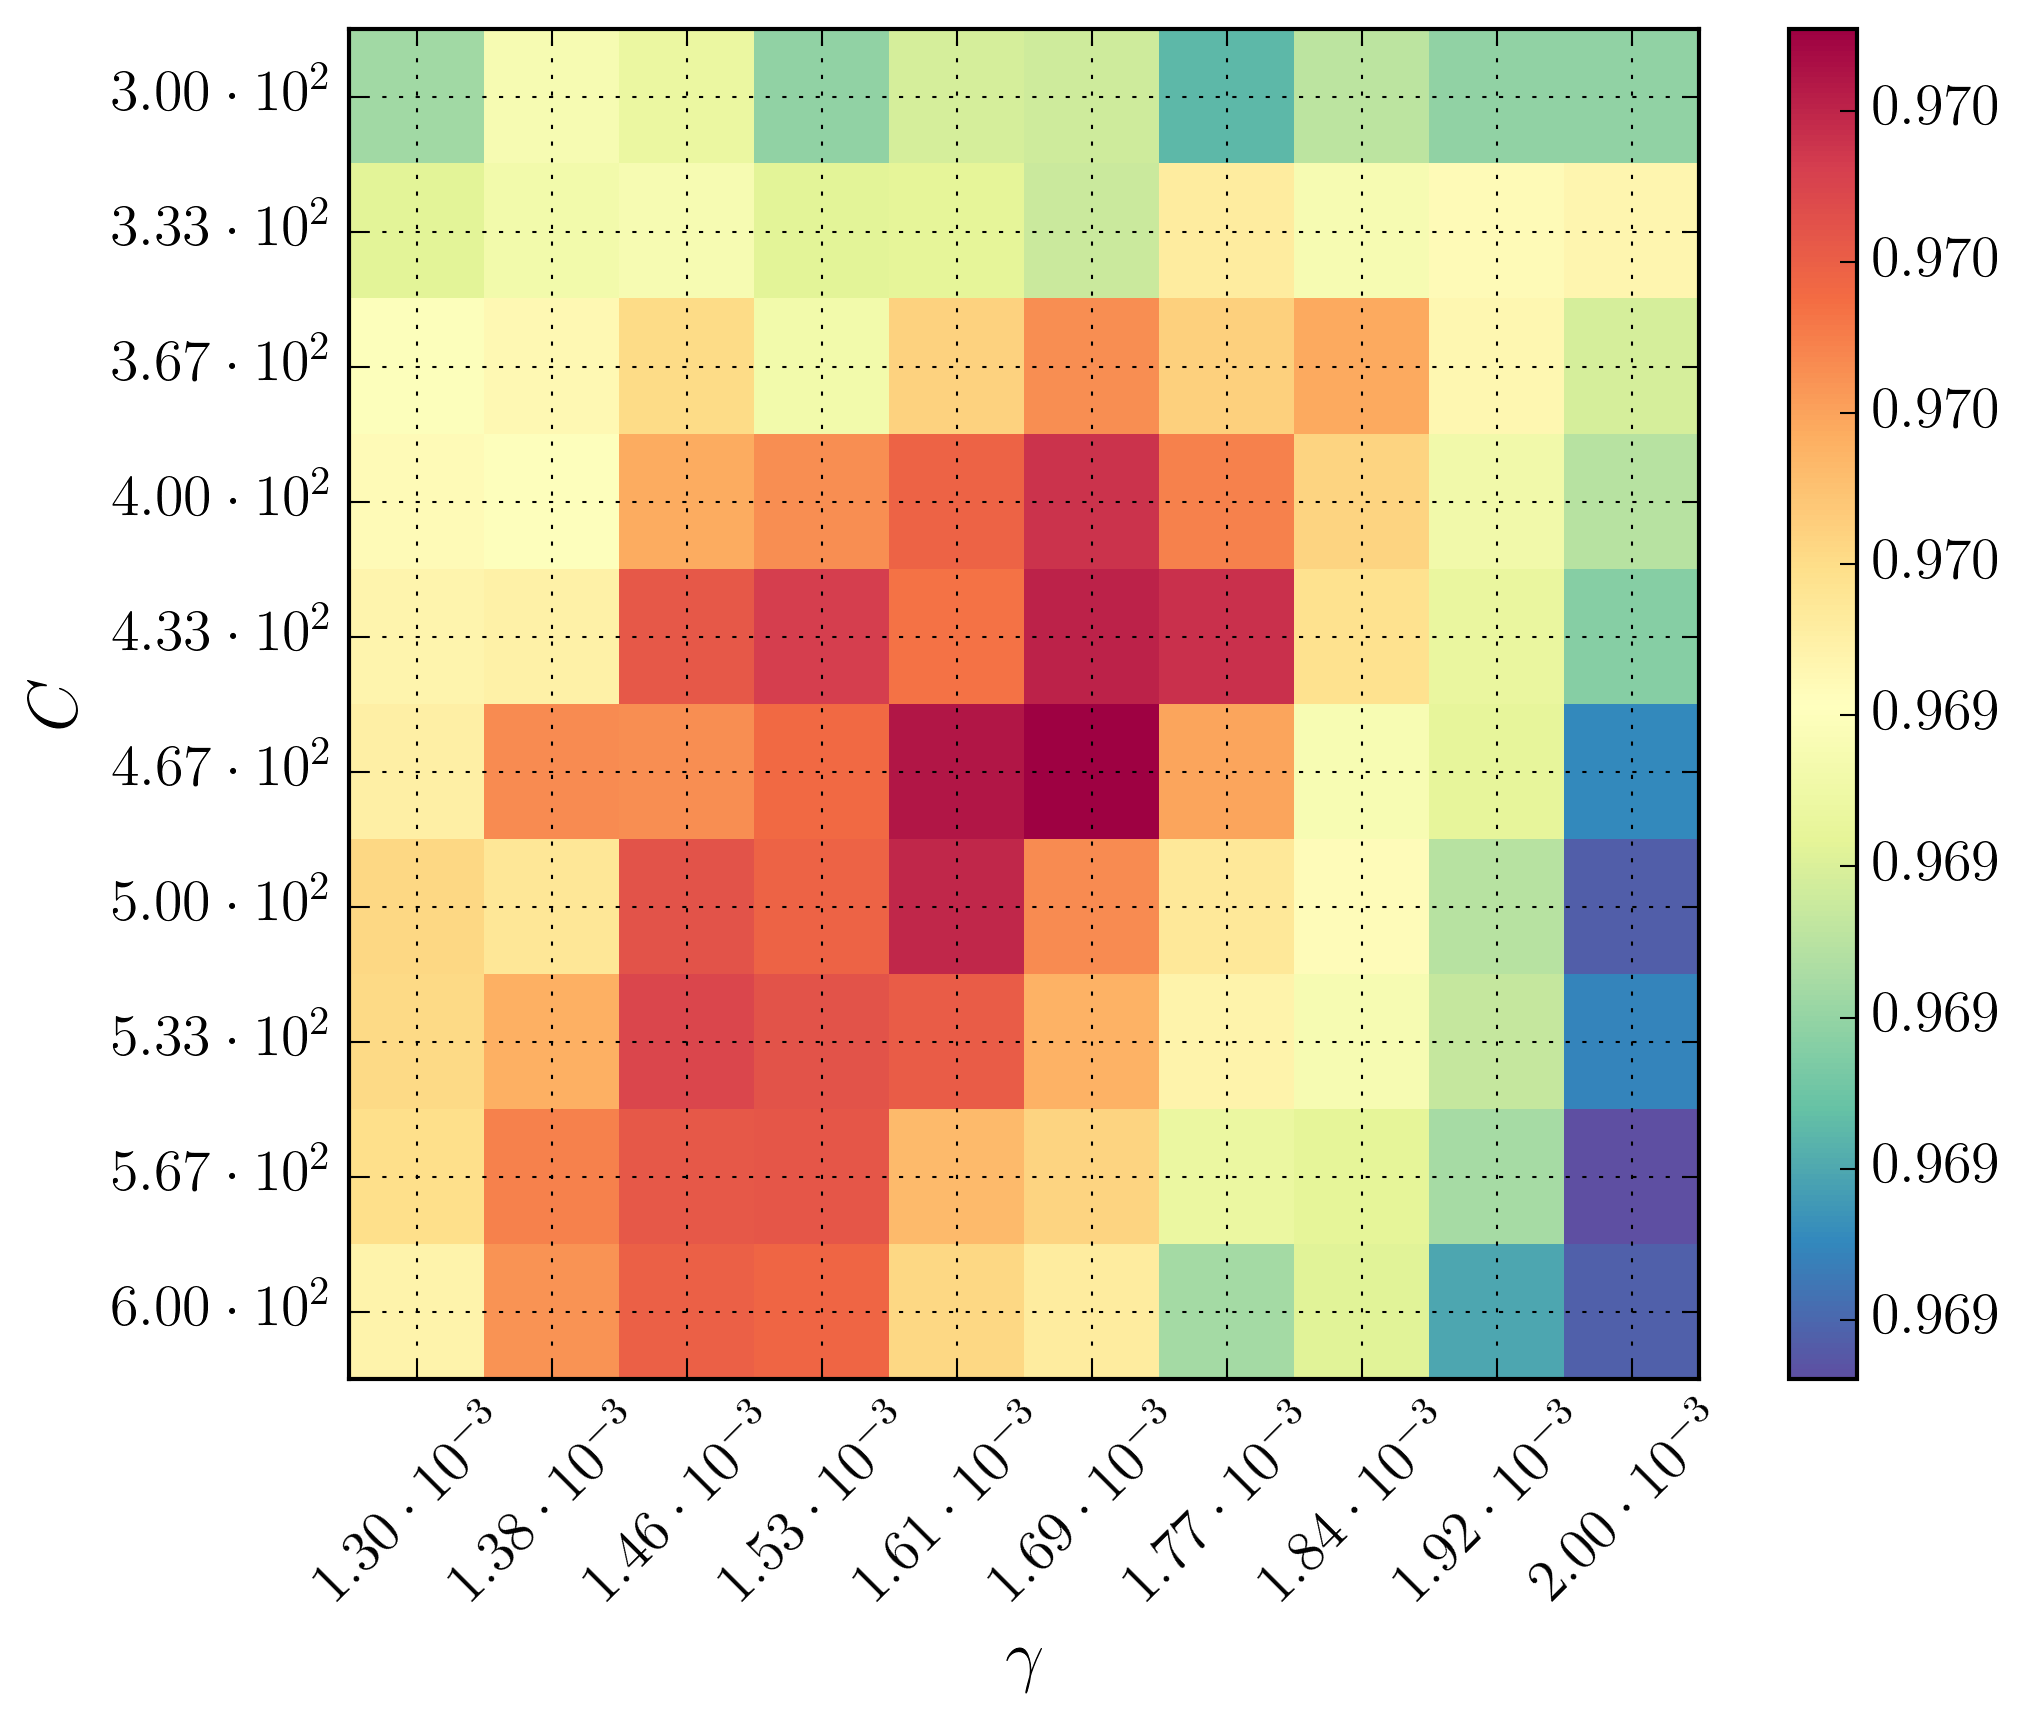
\includegraphics[width=0.51\textwidth,height=0.4\textwidth]{figures/gridsearch/svm/superclasses/svm-superclasses-06.png}}
\hfill
\caption[Hyperparameter optimization for the Support Vector Machine (SVM)]{This figure shows the average, weighted $F_1$ score on the $C$-$\gamma$-plane during the hyperparameter optimization for the Support Vector Machine. We start looking for global optima on a coarse grid with a wide range (upper left), and adjust the grid toward a finer stepwidth. At some point we find an optimum (lower right).}
\label{fig:gridsearch-svm}
\end{figure}

% Hyperparameter optimization
% Add confusion matrix for main classes
% Add confusion matrix for subclasses

\renewcommand{\arraystretch}{1.5}
\resizebox{\textwidth}{!}{
\begin{tabular}{c|ccccccccc|c}
\toprule
%& \multicolumn{8 }{c}{Predicted class} & & \\
%\hline
                   & BV        & CEPH       & DSCT      & EB         & LPV         & NoneVar    & QSO       & RRL        & T2CEPH   & $\Sigma $ \\
\hline
BV                 & {\bf 759} &            &           &     13     &     5       &     16     &      1    &            &     2    &     796   \\
CEPH               &     4     & {\bf 2203} &           &     23     &     8       &     3      &           &     33     &     7    &    2281   \\
DSCT               &           &       5    & {\bf 436} &     16     &             &     24     &           &     30     &          &     511   \\
EB                 &    16     &      20    &     13    & {\bf 3321} &     47      &     62     &      4    &     49     &     6    &    3538   \\
LPV                &     4     &      2     &           &     47     & {\bf 15881} &     58     &      2    &     1      &          &   15995   \\
NoneVar            &    23     &      4     &     21    &     66     &     127     & {\bf 4516} &      30   &     4      &          &    4791   \\
QSO                &     6     &      1     &           &     4      &             &     37     & {\bf 132} &            &          &     180   \\
RRL                &           &      30    &     36    &     79     &      3      &     11     &      1    & {\bf 4307} &     3    &    4470   \\
T2CEPH             &     2     &      27    &           &     12     &      7      &     1      &           &     11     & {\bf 61} &     121   \\
\bottomrule
Recall ($\%$)      &   95.35   &     96.58  &   85.32   &    93.87   &    99.29    &   94.26    &    73.33  &    96.35   &   50.41  &           \\
\hline
Precision ($\%$)   &   93.24   &     96.12  &   86.17   &    92.74   &    98.77    &   95.52    &    77.65  &    97.11   &   77.12  &           \\
\hline
$F_1$ score ($\%$) &   94.28   &     96.35  &   85.74   &    93.30   &    99.00    &   94.89    &    75.43  &    96.73   &   60.97  &           \\
\bottomrule
\end{tabular}
}

\section{Performance of the Random Forest Classifier}

\renewcommand{\arraystretch}{1.5}
\resizebox{\textwidth}{!}{
\begin{tabular}{c|ccccccccc|c}
\toprule
%& \multicolumn{8 }{c}{Predicted class} & & \\
%\hline
                   & BV        & CEPH       & DSCT      & EB         & LPV         & NoneVar    & QSO       & RRL        & T2CEPH   & $\Sigma $ \\
\hline
BV                 & {\bf 775} &      1     &           &     10     &             &      8     &      2    &            &          &     796   \\
CEPH               &     1     & {\bf 2224} &           &     21     &      2      &      5     &           &     23     &          &    2281   \\
DSCT               &           &      2     & {\bf 471} &      5     &             &     26     &           &      7     &          &     511   \\
EB                 &     8     &      12    &           & {\bf 3323} &     48      &     96     &      1    &     47     &     3    &    3538   \\
LPV                &     4     &      3     &           &      8     & {\bf 15943} &     34     &      2    &            &     1    &   15995   \\
NoneVar            &    15     &      3     &     2     &     42     &     94      & {\bf 4624} &     10    &     1      &          &    4791   \\
QSO                &           &            &           &      2     &      3      &     31     & {\bf 143} &     1      &          &     180   \\
RRL                &           &      24    &     5     &     44     &      2      &     15     &           & {\bf 4380} &          &    4470   \\
T2CEPH             &           &      26    &           &     23     &      4      &     2      &           &     6      & {\bf 60} &     121   \\
\bottomrule
Recall ($\%$)      &   97.36   &     97.50  &   92.17   &    93.92   &    99.67    &   96.51    &   79.44   &    97.99   &   49.59  &           \\
\hline
Precision ($\%$)   &   96.51   &     96.91  &   98.54   &    95.54   &    99.05    &   95.52    &   90.51   &    97.99   &   93.75  &           \\
\hline
$F_1$ score ($\%$) &   96.93   &     97.20  &   95.25   &    94.72   &    99.36    &   96.01    &   84.61   &    97.99   &   64.87  &           \\
\bottomrule
\end{tabular}
}

% Hyperparameter optimization
% Add confusion matrix for main classes
% Add confusion matrix for subclasses
% Add feature importance for both

\chapter{Assessing Classification Performance for GAIA}

% Simulating GAIA time series
% Performance of the best classifier on GAIA data